\section{Metodología}

\subsection{Diseño de la representación del problema}

Teniendo en cuenta la definición de una tarea de aprendizaje en robótica, se planteó el modelo del sistema siguiendo la representación propia del RL. En este orden de ideas, se definieron dos agentes independientes entre sí que corresponden al brazo derecho y el brazo izquierdo del robot. Se establece el entorno como el conjunto de articulaciones de los brazos del robot, junto con el resto de la estructura física externa a los dos brazos, ubicadas en el espacio tridimensional con la base del robot centrada en el origen $(0,0,0)$.\\

Siguiendo lo establecido por \textcite{kroemer2021review}, se plantea el problema como una Tarea de Manipulación mediante el enfoque de un Proceso de Decisión de Markov. Así pues, se emplea el enfoque de la definición de un Espacio de Observación tabular y un Espacio de Acción de tipo cartesiano. A continuación, se detallan los elementos fundamentales del planteamiento del problema como un problema de RL:

\begin{enumerate}
	\item \textbf{Espacio de Observación: } En el espacio de observación se definen los estados posibles que puede tener el entorno en cualquier momento de ejecución. En vista de que la cinemática inversa busca determinar los valores de los ángulos articulares, estas mediciones deben formar parte del espacio. 
	
		\begin{table}[h!]
		\centering
		\caption{Descripción de las variables del espacio de observación ($S$)}
		\begin{tabular}{|c|c|}
			\hline
			\textbf{Variable} & \textbf{Descripción} \\
			\hline
			$\theta_1$ & Valor del ángulo en radianes para la articulación \textit{ShoulderPitch} \\
			\hline
			$\theta_2$ & Valor del ángulo en radianes para la articulación \textit{ShoulderRoll} \\
			\hline
			$\theta_3$ & Valor del ángulo en radianes para la articulación \textit{ElbowYaw} \\
			\hline
			$\theta_4$ & Valor del ángulo en radianes para la articulación \textit{ElbowRoll} \\
			\hline
			$\theta_5$ & Valor del ángulo en radianes para la articulación \textit{WristYaw} \\
			\hline
			$e_x$ & Distancia entre posiciones $x_{actual}$ y $x_{goal}$ \\
			\hline
			$e_y$ & Distancia entre posiciones $y_{actual}$ y $y_{goal}$ \\
			\hline
			$e_z$ & Distancia entre posiciones $z_{actual}$ y $z_{goal}$ \\
			\hline
		\end{tabular}
		\label{tab:obs_var}
	\end{table}
	
	Así mismo, por practicidad a la hora de realizar el entrenamiento y para evitar sesgar al agente para que tome una ruta en particular o la priorice sobre otra, se recurre a integrar el valor del error en las tres direcciones cartesianas rectangulares con el objetivo de poder realizar una medición de la distancia entre la posición en la que se encuentra el efector final en un momento dado y la posición esperada, para así realizar un ajuste o determinar la ocurrencia de un éxito. La estructura del espacio de observación se muestra en la Tabla \ref{tab:obs_var} y los rangos de cada variable a continuación:
	
	\begin{table}[h!]
		\centering
		\caption{Rangos de valores para cada variable por brazo}
		\begin{tabular}{|c|c|c|}
			\hline
			\textbf{Variable} & \textbf{Rango (Izquierdo)} & \textbf{Rango (Derecho)} \\
			\hline
			$\theta_1$ & $[-2.0857, 2.0857] \text{ rad}$ & $[-2.0857, 2.0857] \text{ rad}$ \\
			\hline
			$\theta_2$ & $[0.0087, 1.5620] \text{ rad}$ & $[-1.5620, -0.0087] \text{ rad}$ \\
			\hline
			$\theta_3$ & $[-2.0857, 2.0857] \text{ rad}$ & $[-2.0857, 2.0857] \text{ rad}$ \\
			\hline
			$\theta_4$ & $[-1.3614, -0.0087] \text{ rad}$ & $[0.0087, 1.3614] \text{ rad}$ \\
			\hline
			$\theta_5$ & $[-1.8239, 1.8239] \text{ rad}$ & $[-1.8239, 1.8239] \text{ rad}$ \\
			\hline
			$e_x$ & $[-\infty, +\infty] \text{ m}$ & $[-\infty, +\infty] \text{ m}$ \\
			\hline
			$e_y$ & $[-\infty, +\infty] \text{ m}$ & $[-\infty, +\infty] \text{ m}$ \\
			\hline
			$e_z$ & $[-\infty, +\infty] \text{ m}$ & $[-\infty, +\infty] \text{ m}$ \\
			\hline
		\end{tabular}
		\label{tab:obs_rangos}
	\end{table}
	
	
	\item \textbf{Espacio de Acción: } En el espacio de acción se definen las posibles acciones que toman los agentes. De esta manera, como el objetivo principal consiste en alterar los valores de los ángulos en cada ejecución, se codifica los cambios que se le deben aplicar a cada ángulo en un paso. El agente tiene la potestad de decidir si aplica una o varias acciones en un paso específico. Los valores establecidos como límites máximo y mínimo buscan asegurar que el movimiento en cada paso sea suave y así reducir un posible daño en el robot e incluso permitiendo tiempo de reacción de emergencia en caso de ser necesario. La estructura del espacio de acción es la siguiente:
	
	\begin{table}[h!]
		\centering
		\caption{Descripción del espacio de acción ($A$) para cualquier brazo}
		\begin{tabular}{|c|c|}
			\hline
			\textbf{Acción} & \textbf{Rango} \\
			\hline
			$\Delta\theta_1$ & $[-0.50, 0.50] \text{ rad}$ \\
			\hline
			$\Delta\theta_2$ & $[-0.50, 0.50] \text{ rad}$ \\
			\hline
			$\Delta\theta_3$ & $[-0.50, 0.50] \text{ rad}$ \\
			\hline
			$\Delta\theta_4$ & $[-0.50, 0.50] \text{ rad}$ \\
			\hline
			$\Delta\theta_5$ & $[-0.50, 0.50] \text{ rad}$ \\
			\hline
		\end{tabular}
		\label{tab:accion_space}
	\end{table}
	
	\item \textbf{Función de Recompensa: } La función de recompensa se diseña para establecer las aportaciones y penalizaciones compuestas que debe recibir el agente en cada paso del entrenamiento para evaluar la correctitud de la política vigente que se está explotando en ese momento. La función se diseñó a partir de ajustes experimentales buscando favorecer determinados comportamientos sobre otros, particularmente, el acercamiento al punto objetivo por parte del efector final y la ocurrencia de un éxito, definido este como un error menor a 2cm. Matemáticamente, se puede expresar de la siguiente manera:
	
	\begin{equation}
		r_n(s) = \sum_{k} R_n^{k}
	\end{equation}
	
	donde corresponde a la sumatoria de un conjunto de funciones parciales que calculan penalizaciones y contribuciones según los criterios:
	\begin{itemize}
		\item Mejoramiento del error respecto al paso inmediatamente anterior. Es decir, si el efector final se ha acercado más a la posición esperada.
		
		\begin{equation}
			R_{n}^{\text{improvement}} = 30 \cdot (d_{n-1} - d_{n})
		\end{equation}
		
		\item Penalización constante dependiendo del error (medido como la distancia euclidiana entre la posición del efector final y la posición deseada) calculado a partir de las mediciones de los errores unidimensionales en el espacio de observación como $d_n = \sqrt{e_x^2 + e_y^2 + e_z^2}$.
		
		\begin{equation}
			R_{n}^{\text{proximity}} = -2.0 \cdot d_n
		\end{equation}
		
		\item Suavidad de los movimientos del brazo, penalizado de forma constante dependiendo de qué tan extremos son las variaciones de los ángulos articulares en la contribución total de las acciones por cada paso.
		
		\begin{equation}
			R_{n}^{\text{smoothness}} = -0.15 \cdot \left|\Delta\theta\right|^2
		\end{equation}
		
		\item Penalización por alcanzar los límites de alguno de los ángulos articulares con una tolerancia de $\pm 1.0\times10^{-6}$, en cuyo caso se le quita a la recompensa total. Este término surge de la necesidad de proteger la operatividad del robot y evitar que alcance ángulos por fuera de lo permitido por la configuración del hardware y los mecanismos que permiten el movimiento adecuado del brazo. 
		
		\begin{equation}
			R_{n}^{\text{limit}} =
			\begin{cases}
				-0.75 & \text{si } \theta_i = \theta_{i,\min} \lor \theta_i = \theta_{i,\max} \quad \forall i \in \{1,2,3,4,5\} \\
				0 & \text{de lo contrario}
			\end{cases}
		\end{equation}
		
		\item Finalmente, una recompensa especial por alcanzar una posición final con un error menor a 2cm, el cual fue definido como el valor del umbral del éxito durante entrenamiento. Esta recompensa busca asegurar que el agente no pierda de vista el objetivo primordial que es alcanzar la posición final deseada. Se estableció el valor de 2cm puesto que en la práctica corresponde a una diferencia poco significativa que permitiría, en la mayoría de casos, aprovechar la configuración alcanzada para realizar alguna tarea local como agarrar un objeto, por ejemplo.
		
		\begin{equation}
			R_{n}^{\text{success}} =
			\begin{cases}
				25.0 & \text{si } d_n \leq 0.02 \\
				0 & \text{de lo contrario}
			\end{cases}
		\end{equation}
		
	\end{itemize}
	
	\item \textbf{Currículo: } El planteamiento del método de currículo se realizó a partir de las técnicas expuestas por \textcite{weng2020curriculum}. Se decidió emplear la técnica de Generación Automática de Objetivos y como estrategia para realizar el agrupamiento de los objetivos definidos por nivel de dificultad, se utilizó una medida que se optó por denominar como \textbf{Radio de Currículo}.\\
	
	El radio de currículo define una zona esférica alrededor del objetivo dentro de la cual se inicializa la posición del efector final al comienzo de cada episodio de entrenamiento. Al inicio, el radio es pequeño arrancando con un valor de 10cm, lo que implica que el robot comienza cerca del objetivo. Así se facilita el aprendizaje de movimientos básicos al inicio del entrenamiento. A medida que el agente mejora su desempeño, el radio se incrementa gradualmente, presentando desafíos más complejos al alejar la posición inicial del objetivo. Esta técnica permite que el robot construya sus habilidades de forma escalonada, promoviendo una convergencia más estable y eficiente hacia políticas de control más generalizadas.\\
	
	En este diseño, el radio del currículo inicia con un valor de 0.00 y automáticamente incrementa de a 10cm una vez que se hayan alcanzado 5 intentos exitosos consecutivos con un mismo radio. El tener 5 éxitos consecutivos asegura que la política aprendida hasta entonces ha logrado superar adecuadamente el desafío de alcanzar las poses finales para el nivel de dificultad propuesto hasta entonces. El valor del radio del currículo $c$ por cada nivel $k$ viene dado por:
	
	$$
		c_k = \min(c_{k-1}+\Delta c, c_{\max})
	$$
	
	donde se reitera que $\Delta c = 0.1$ y $c_{\max} = 0.51$, ambas expresadas en metros, que corresponde a la media de distancia entre todos los puntos factibles alcanzables en los espacios de trabajo de ambos brazos, los cuales se mostrarán en simulación más adelante.
	
\end{enumerate}


\subsection{Entrenamiento con sintonización de hiperparámetros}

Una vez definido el modelo del problema, con la definición de los agentes, los espacios de observación y acción, la función de recompensa y la técnica de incremento curricular, el siguiente paso a seguir consiste en establecer la forma de entrenar. Se planteó el uso de dos algoritmos diferentes, PPO y SAC, para realizar una comparación entre el resultado de ambos. Esta decisión se tomó por dos motivos: en primer lugar, la oportunidad de comparar el desempeño entre un algoritmo basado en política como PPO y un algoritmo basado en valor como SAC para ver cuál enfoque resulta mejor en el problema en cuestión. El montaje del entorno aprovechó el ambiente orientado al RL Gymnasium introducido por \textcite{towers2024gymnasium}, que permite programar entornos personalizados acorde al planteamiento conceptual de los mismos.\\

En segundo lugar, los dos algoritmos seleccionados tienen una implementación existente de código abierto realizada por \textcite{raffin2021stable} como parte del framework Stable Baselines 3, el cual está diseñado específicamente para facilitar la programación de tareas relacionadas con RL. Stable Baselines tiene incorporados métodos orientados al entrenamiento, aleatorización de muestras, guardado de políticas y carga de las mismas en formatos de archivo compatibles con su sistema de codificación interno y también con el ambiente de Gymnasium así como sus definiciones de entornos personalizados \parencite{raffin2021stable}.\\

Como la implementación de los algoritmos mencionados en Stable Baselines 3 tiene una serie de hiperparámetros ajustables que pueden cambiar sustancialmente los resultados de entrenamiento de una política, se acudió al framework de optimización de hiperparámetros Optuna presentado por \textcite{optuna_2019}. Optuna es capaz de realizar estudios de optimización sobre un espacio de hiperparámetros especificados junto con su rango discreto y/o categórico de valores posibles. Optuna se encarga de seleccionar valores factibles dentro del rango especificado y configurar instancias de los algoritmos con dichos hiperparámetros. Finalmente, la herramienta emplea la maximización de la recompensa notificada por el entorno para seleccionar el mejor de los estudios asociado a la mejor combinación de hiperparámetros y, por ende, la mejor política aprendida.\\

Para el caso de los algoritmos PPO y SAC, se establecieron las siguientes referencias para configurar los estudios de Optuna y realizar \textit{trials} de entrenamiento de manera secuencial:

\begin{table}[h!]
	\centering
	\caption{Espacio de hiperparámetros explorado para PPO}
	\begin{tabular}{|l|c|l|}
		\hline
		\textbf{Hiperparámetro} & \textbf{Tipo} & \textbf{Rango de valores} \\
		\hline
		\texttt{learning\_rate} & Float & $[1\times10^{-5}, 1\times10^{-3}]$ \\
		\texttt{n\_steps} & Categórico & \{256, 512, 1024, 2048\} \\
		\texttt{gamma} & Float & $[0.9, 0.9999]$ \\
		\texttt{gae\_lambda} & Float & $[0.8, 0.99]$ \\
		\texttt{ent\_coef} & Float & $[1\times10^{-8}, 1\times10^{-1}]$ \\
		\texttt{clip\_range} & Float & $[0.1, 0.4]$ \\
		\texttt{vf\_coef} & Float & $[0.1, 1.0]$ \\
		\texttt{batch\_size} & Categórico & \{64, 128, 256\} \\
		\hline
	\end{tabular}
	\label{tab:optuna-ppo}
\end{table}

\begin{table}[h!]
	\centering
	\caption{Espacio de hiperparámetros explorado para SAC}
	\begin{tabular}{|l|c|l|}
		\hline
		\textbf{Hiperparámetro} & \textbf{Tipo} & \textbf{Rango de valores} \\
		\hline
		\texttt{learning\_rate} & Float & $[1\times10^{-5}, 1\times10^{-3}]$ \\
		\texttt{buffer\_size} & Categórico & \{100000, 300000, 1000000\} \\
		\texttt{batch\_size} & Categórico & \{128, 256, 512\} \\
		\texttt{tau} & Float & $[0.005, 0.05]$ \\
		\texttt{gamma} & Float & $[0.9, 0.9999]$ \\
		\texttt{train\_freq} & Categórico & \{1, 4, 8, 16\} \\
		\texttt{gradient\_steps} & Categórico & \{-1, 1, 4, 8, 16\} \\
		\texttt{ent\_coef} & Fijo & 'auto' \\
		\hline
	\end{tabular}
	\label{tab:optuna-sac}
\end{table}

Finalmente, para ejecutar los estudios de Optuna de manera eficiente, se utilizó la táctica del Entrenamiento sobre Modelo Surrogado. Básicamente, esta consiste en crear una copia del entorno con menos restricciones o menor especificidad para que los episodios de entrenamiento se puedan ejecutar con mayor velocidad. Esta táctica permite ahorrar tiempo de entrenamiento y permitir el completamiento de una mayor cantidad de \textit{trials} de Optuna en la ventana de timeout, la cual se estableció en 8 horas para cada agente.\\

En este caso, la simplificación del entorno consistió en suprimir el modelo del agente sobre el mundo simulado. Así, el modelo surrogado consistió en una copia netamente matemáticamente del modelo completo, sobre la cual no se consideran los efectos de la física del robot sino solamente las mediciones observables en el espacio de observación y los cálculos de posicionamiento realizables con estos valores para determinar los errores, e igualmente compatible con Gymnasium \parencite{towers2024gymnasium}. La ventaja de esta táctica es que, sin pérdida de generalidad, la política aprendida tiene exactamente el mismo comportamiento, pero vinculado a tiempo del computador en lugar del tiempo simulado del movimiento del robot físico. En este proyecto, cada entrenamiento se realizó sobre 1.000.000 de timesteps. \\

\subsection{Visualización mediante simulación}

Para visualizar el comportamiento del robot y de los brazos entrenados se acudió a un simulador de código abierto qiBullet desarrollado por \textcite{busy2019qibullet}. La utilidad de qiBullet se refleja en que permite simular fielmente la física del entorno como el valor de la gravedad, torque, control de motores y velocidades de movimiento de los componentes de los robots de Softbank Robotics, teniendo modelos URDF de Pepper, Nao y Romeo. En el caso de este proyecto, se empleó el modelo URDF de Pepper. Por otro lado, aprovechando la flexiblidad de Gymnasium, se construyeron entornos compatibles con qiBullet \parencite{towers2024gymnasium}.\\

El proceso de instalación y configuración de qiBullet se encuentra disponible en la Wiki del repositorio oficial \footnote{\url{https://github.com/softbankrobotics-research/qibullet/wiki}}. Una vez instalado, existen archivos de prueba que pueden resultar útiles para verificar el correcto funcionamiento de la simulación y para familiarizarse con la orientación del robot materializado en el entorno básico e incluso probar interacción manualmente con el mouse. \\

\begin{figure}[h!]
	\centering
	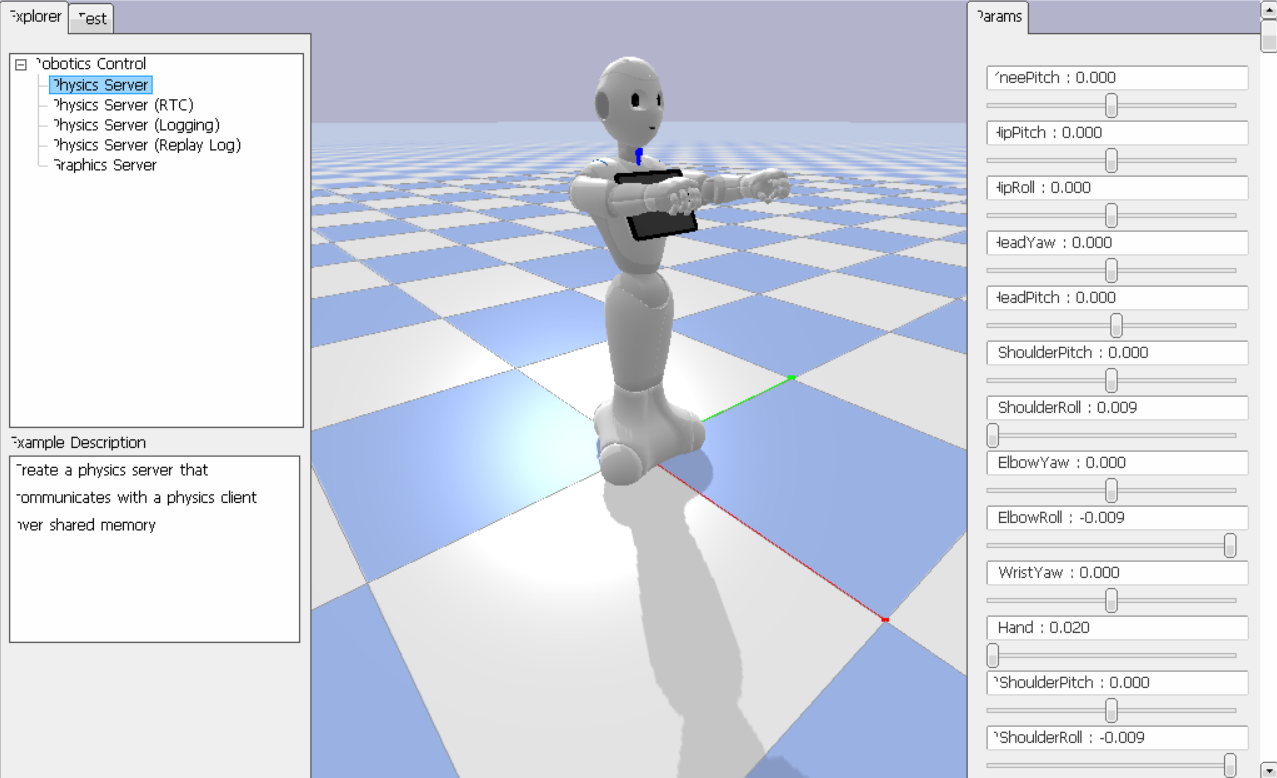
\includegraphics[width=350pt]{images/metodologia/qibullet}
	\caption{Ejecución local del simulador qiBullet con un modelo del robot Pepper}
	\label{fig:qibullet}
\end{figure}

El simulador de qiBullet fue utilizado, además, para generar una visualización del espacio de trabajo de los brazos del robot. Para generar el espacio de trabajo del robot, se recurrió al método de muestreo aleatorio basado en puntos. De esta manera, considerando los rangos útiles de las articulaciones del robot presentados en la Tabla \ref{tab:obs_rangos}, se realizan selecciones aleatorias y se utilizan las ecuaciones de cinemática directa para calcular la posición del efector final y mapearla sobre la simulación para mejorar la apreciación del espacio alcanzable por cada brazo.\\

En total, se realiza un muestreo de 8 repeticiones, lo cual resulta en $8^5 = 32065$ configuraciones posibles que se mapean por cada brazo. Estos puntos finales son conservados en una estructura de datos en memoria para poder acceder a ella durante el entrenamiento y durante las pruebas. Los puntos objetivo para un radio de currículo específico se seleccionan desde este conjunto de puntos alcanzables, así como los puntos para realización de pruebas con las mejores políticas.\\

Cabe resaltar que, en simulación, la posición del efector final medida se ubica en lo que corresponde al inicio de la muñeca del brazo. Técnicamente, es el extremo inicial del efector final en lugar del extremo final. Sin embargo, para simplificar el modelo se prefirió utilizar esta coordenada para realizar los cálculos de error sin contemplar el offset relacionado a la longitud de la mano de 6.950 cm (sobre el eje x de su sistema local de referencia) de acuerdo con la documentación oficial del robot \parencite{softbank2023pepper}. \\

\begin{figure}[h!]
	\centering
	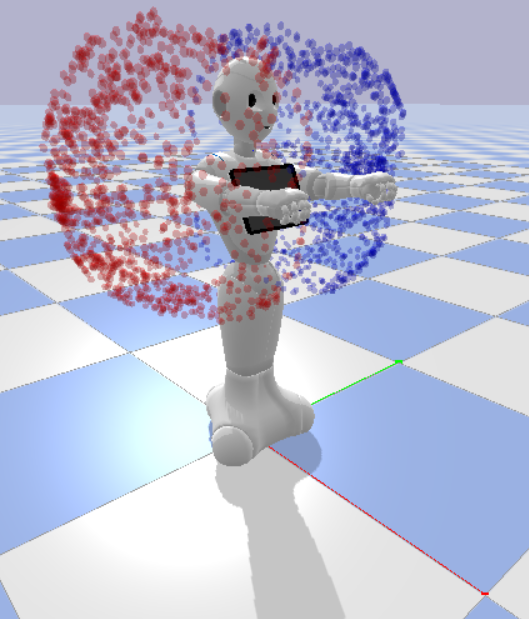
\includegraphics[width=200pt]{images/metodologia/workspace}
	\caption{Visualización del espacio de trabajo alcanzable de cada brazo superpuesto a la simulación. Los puntos en azul muestran el espacio de trabajo del brazo izquierdo y los rojos el del brazo derecho.}
	\label{fig:workspace}
\end{figure}

Esta ubicación de la coordenada de medición se puede apreciar en la Figura \ref{fig:workspace}, donde se el ángulo en el cual está orientada la visualización deja ver que los puntos que muestrean la pose estándar con todos los ángulos en cero, se encuentran sobre las muñecas en ambos brazos.


\subsection{Ejecución de pruebas de funcionamiento}

La ejecución de las pruebas de funcionamiento se realizó siguiendo el protocolo descrito a continuación:

\begin{enumerate}
	\item Generar un archivo de caché donde se almacenan los puntos muestreados del espacio de trabajo factible. Si el archivo ya existe, aprovecharlo y cargar los puntos en memoria.
	
	\item Seleccionar aleatoriamente 1000 puntos del espacio de trabajo.
	
	\item Iniciar un episodio de máximo 250 timesteps con el robot posicionado en una pose aleatoria diferente a la pose de destino, a partir de los métodos de Gymnasium.
	
	\item Reproducir la política en proceso de prueba con el agente entrenado (brazo izquierdo o brazo derecho) hasta que se alcance una posición final ubicada a una distancia menor que el umbral de precisión configurado.
	
	\item La ejecución de la prueba calcula la media y el error de precisión de la distancia entre la posición del efector final y la posición deseada. Además, retorna un conteo de la cantidad de episodios exitosos dentro de las pruebas realizadas.
\end{enumerate}

Nuevamente, para agilizar el proceso de pruebas se diseñó un argumento de ejecución que permite realizar el lanzamiento de la ráfaga de pruebas con interfaz gráfica (mostrando el movimiento en el simulador) o en consola (mostrando simplemente el resultado de cada prueba y la cantidad de episodios necesarios para llegar a la posición considerada como éxito).\\

En la Figura \ref{fig:test-gui} se muestra cómo se visualiza una prueba con interfaz gráfica. El robot inicia en una posición diferente a la de destino y realiza un movimiento de sus articulaciones permaneciendo estático en las demás articulaciones (base, torso y cabeza) hasta llegar a la posición esperada, indicada con un punto, como se ve en la Figura \ref{fig:test-start}. Una vez que llega a la posición deseada dentro del margen de precisión esperado, el punto desaparece y permite ver la pose final del robot para lograr el objetivo, como se aprecia en la Figura \ref{fig:test-reached}. De lo contrario, si no es exitosa, automáticamente se reinicia el entorno de Gymnasium e inicia la siguiente prueba.

\begin{figure}[h!]
	\centering
	
	\begin{subfigure}[b]{0.45\textwidth}
		\centering
		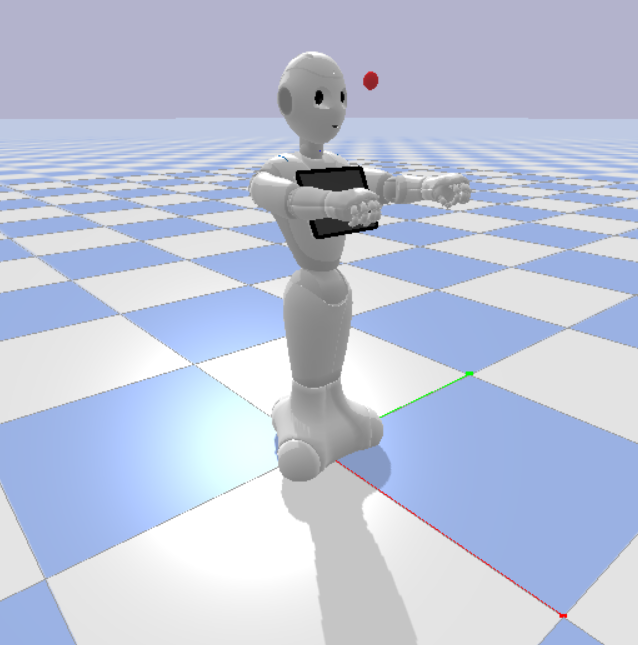
\includegraphics[width=\textwidth]{images/metodologia/test_start}
		\caption{Estado inicial de una prueba}
		\label{fig:test-start}
	\end{subfigure}
	\hfill
	\begin{subfigure}[b]{0.465\textwidth}
		\centering
		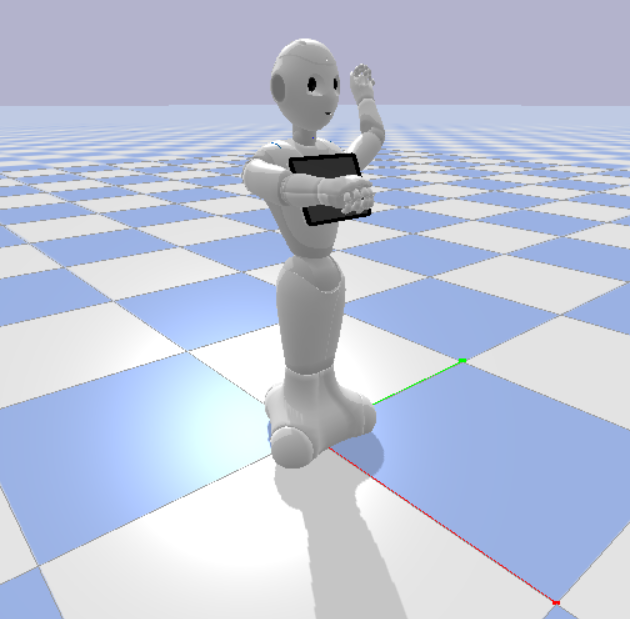
\includegraphics[width=\textwidth]{images/metodologia/test_reached}
		\caption{Estado exitoso de una prueba}
		\label{fig:test-reached}
	\end{subfigure}
	
	\caption{Estados de ejecución de una prueba con interfaz gráfica. El punto rojo muestra la posición deseada representada en el sistema de coordenadas global: en este caso, el punto $(x,y,z)=(-0.22, 0.41, 1.16) \text{ m}$.}
	\label{fig:test-gui}
\end{figure}